\documentclass[supercite]{sample}

\title{~~~~~~计算机视觉结课报告~~~~~~}
\author{张隽翊}
\school{计算机科学与技术学院}
\classnum{CS2003}
\stunum{U202015374}
\instructor{李贤芝}
\date{2023年5月4日}
\hypersetup{
colorlinks=true,
linkcolor=black
}
\usepackage{listings}
\usepackage{algorithm, multirow}
\usepackage{algpseudocode}
\usepackage{amsmath}
\usepackage{makecell}
\usepackage{amsthm}
\usepackage{framed}
\usepackage{mathtools}
\usepackage{subcaption}
\usepackage{xltxtra} %提供了针对XeTeX的改进并且加入了XeTeX的LOGO, 自动调用xunicode宏包(提供Unicode字符宏)
\usepackage{bm}
\usepackage{tikz}
\usepackage{tikzscale}
\usepackage{pgfplots}
%\usepackage{enumerate}

\pgfplotsset{compat=1.16}
\definecolor{dkgreen}{rgb}{0,0.6,0}
\definecolor{gray}{rgb}{0.5,0.5,0.5}
\definecolor{mauve}{rgb}{0.58,0,0.82}
\lstset{frame=tb,
  language=Go,
  aboveskip=3mm,
  belowskip=3mm,
  showstringspaces=false,
  columns=flexible,
  basicstyle={\small\ttfamily},
  numbers=none,
  numberstyle=\tiny\color{gray},
  keywordstyle=\color{blue},
  commentstyle=\color{dkgreen},
  stringstyle=\color{mauve},
  breaklines=true,
  breakatwhitespace=true,
  tabsize=3
}
\newcommand{\cfig}[3]{
  \begin{figure}[htb]
    \centering
    \includegraphics[width=#2\textwidth]{images/#1.tikz}
    \caption{#3}
    \label{fig:#1}
  \end{figure}
}

\newcommand{\sfig}[3]{
  \begin{subfigure}[b]{#2\textwidth}
    \includegraphics[width=\textwidth]{images/#1.tikz}
    \caption{#3}
    \label{fig:#1}
  \end{subfigure}
}

\newcommand{\xfig}[3]{
  \begin{figure}[htb]
    \centering
    #3
    \caption{#2}
    \label{fig:#1}
  \end{figure}
}

\newcommand{\rfig}[1]{\autoref{fig:#1}}
\newcommand{\ralg}[1]{\autoref{alg:#1}}
\newcommand{\rthm}[1]{\autoref{thm:#1}}
\newcommand{\rlem}[1]{\autoref{lem:#1}}
\newcommand{\reqn}[1]{\autoref{eqn:#1}}
\newcommand{\rtbl}[1]{\autoref{tbl:#1}}

\algnewcommand\Null{\textsc{null }}
\algnewcommand\algorithmicinput{\textbf{Input:}}
\algnewcommand\Input{\item[\algorithmicinput]}
\algnewcommand\algorithmicoutput{\textbf{Output:}}
\algnewcommand\Output{\item[\algorithmicoutput]}
\algnewcommand\algorithmicbreak{\textbf{break}}
\algnewcommand\Break{\algorithmicbreak}
\algnewcommand\algorithmiccontinue{\textbf{continue}}
\algnewcommand\Continue{\algorithmiccontinue}
\algnewcommand{\LeftCom}[1]{\State $\triangleright$ #1}

\newtheorem{thm}{定理}[section]
\newtheorem{lem}{引理}[section]

\colorlet{shadecolor}{black!15}

\theoremstyle{definition}
\newtheorem{alg}{算法}[section]

\def\thmautorefname~#1\null{定理~#1~\null}
\def\lemautorefname~#1\null{引理~#1~\null}
\def\algautorefname~#1\null{算法~#1~\null}

\begin{document}

\maketitle

\clearpage

\pagenumbering{Roman}

\tableofcontents[level=2]

\clearpage

\pagenumbering{arabic}

\section{目标检测任务概述}

\subsection{目标检测任务简介}

目标检测 (Detection) 是计算机视觉的基本任务之一,旨在从一副图像上用矩形框把一些物体框定出来。不同于分类 (Classification) 任务关注整体图片类别,目标检测关注的是特定的物体目标,要求在图片中同时识别出目标物的类别信息和位置信息,是一个 classification + localization 的问题。分类给出的是整张图片的内容描述,而检测给出的则是对图片前景和背景的理解。对于检测人物,我们需要从背景中分离出感兴趣的目标,并确定这一目标的描述,即类别和位置。检测模型的输出形式通常是一个列表,列表的每一项使用一个数组给出检出目标的类别和位置,常用矩形检测框的坐标表示。

\subsection{目标检测历史研究}

\subsubsection{深度学习时代之前}

早期的目标检测流程分为三步:候选框生成、特征向量提取和区域分类。

\begin{enumerate}
	\renewcommand{\labelenumi}{\theenumi)}
	\item 第一阶段:候选框生成。这一阶段的目标是搜索图像中可能包含对象的位置,又叫感兴趣区域 (ROI, region of interest)。直观的思路是用滑动窗口扫描整幅图像。为了捕捉不同尺寸和不同宽高比对象的信息,输入图像被重新分割为不同的尺寸,然后用不同尺寸的窗口滑动经过输入图像;
	\item 第二阶段:特征向量提取。在图像的每个位置上利用滑动窗口获取固定长度的特征向量,从而捕捉该区域的判别语义信息。该特征向量通常由低级视觉描述子编码而成,包括 SIFT (Scale Invariant Feature Transform)、HOG (Histogram of Gradients)、SURF (Speeded Up Robust Features) 等,它们对缩放、光线变化和旋转具备一定的鲁棒性;
	\item 第三阶段:区域分类。学习区域分类器,为特定区域分配类别标签。
\end{enumerate}

通常会使用支持向量机 (SVM, support vector machine),因为它在小规模训练数据上性能优异。此外,Bagging、Cascade Learning 和 Adaboost 等分类技术也会用在区域分类阶段,帮助提高目标检测的准确率。

\subsubsection{深度学习时代之后}

在将深度卷积神经网络成功应用于图像分类后,基于深度学习技术的目标检测也取得了巨大进步,并且基于深度学习的新算法显著优于传统的目标检测算法。

目前,基于深度学习的目标检测框架可以分为两大类:

\begin{enumerate}
	\renewcommand{\labelenumi}{\theenumi)}
	\item 二阶检测器 (Two-stage):如基于区域的 CNN (R-CNN) 及其变体;
	\item 一阶检测器 (One-stage):如 YOLO 及其变体。
\end{enumerate}

二阶检测器首先使用候选框生成器生成稀疏的候选框集,并从每个候选框中提取特征;然后使用区域分类器预测候选框区域的类别。一阶检测器直接对特征图上每个位置的对象进行类别预测,不经过二阶检测中的区域分类步骤。两者的结构如图\ref{fig1-1}所示。

\begin{figure}[htb] % here top bottom
	\begin{center}
		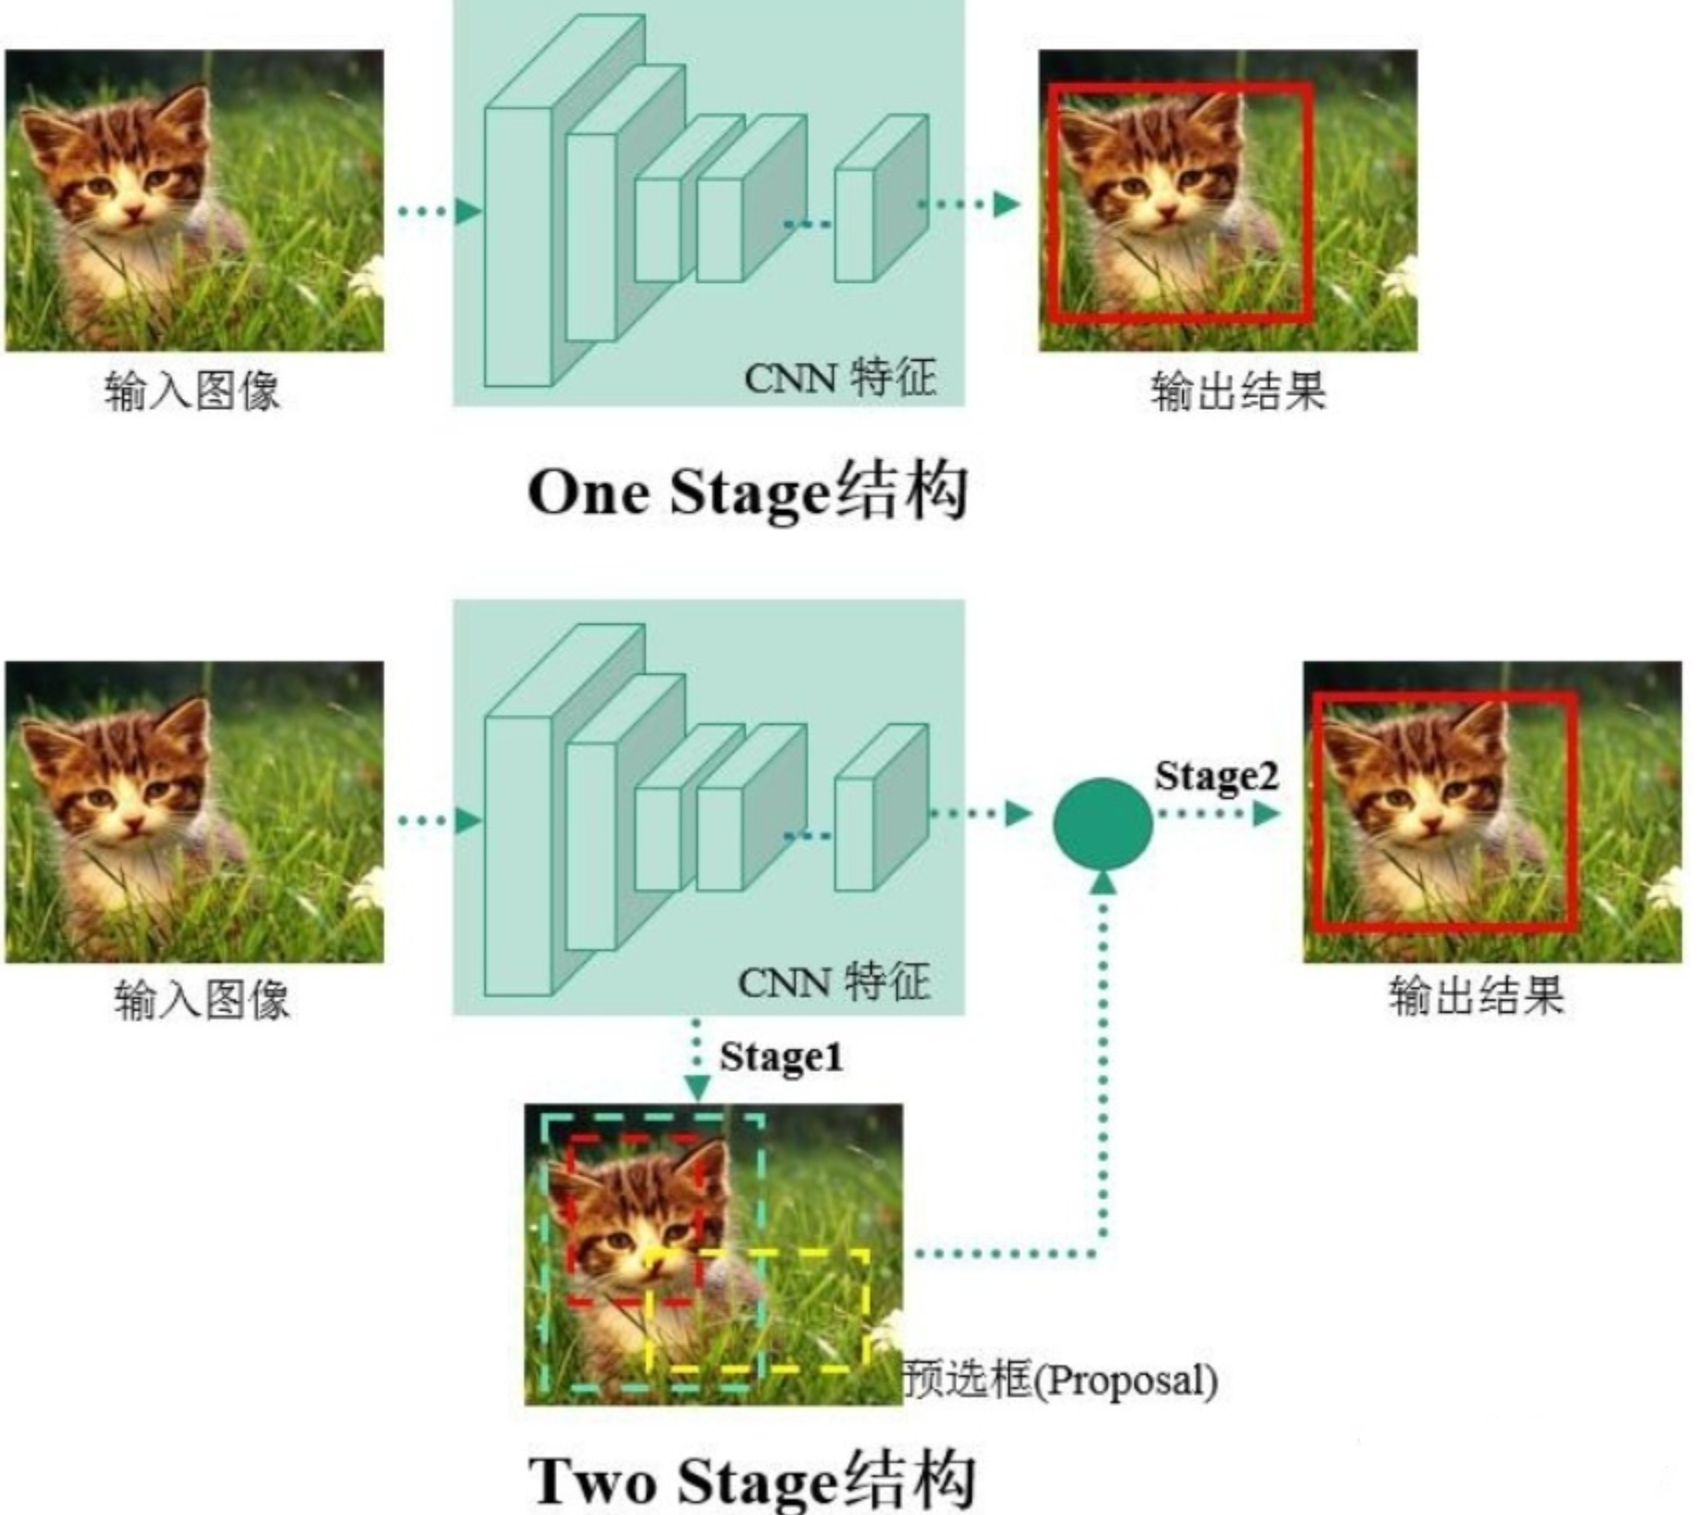
\includegraphics[scale=0.20]{images/1-1.png}
		\caption{One Stage 和 Two Stage 结构对比}
		\label{fig1-1}
	\end{center}
\end{figure}

通常而言,二阶检测器的性能更好,在公开基准上取得了当前最优结果,而一阶检测器更省时,在实时目标检测方面具备更强的适用性。

\section{两阶段目标检测典型算法}

两阶段模型也称为基于区域 (Region-based) 的方法,我们选取 R-CNN 系列工作作为这一类型的代表,典型网络包括 R-CNN、Fast R-CNN、Faster R-CNN 以及 Mask R-CNN。下面我将结合原始论文和自己的理解简述每种网络的基本原理,以及后一种网络相比前一种网络有哪些技术上的改进。

\subsection{R-CNN}

R-CNN (Regions with Convolutional Neural Networks) 是一种经典的目标检测算法,其基本原理是先使用选择性搜索算法在输入图像中提取候选区域,然后对每个候选区域进行卷积特征提取,最后使用支持向量机 (SVM) 分类器来判断该区域内是否包含目标对象。R-CNN 的缺点是速度慢,因为需要对每个候选区域分别进行卷积特征提取和分类器判断。

\subsection{Fast R-CNN}

Fast R-CNN 是对 R-CNN 的改进,它将整张图像输入卷积神经网络中,提取出一组共享的卷积特征图。然后,使用 ROI Pooling 将每个候选区域投影到特征图上,以提取出该区域内的特征向量。最后,将特征向量输入全连接层进行分类和回归。Fast R-CNN 相较于 R-CNN,速度更快,因为卷积特征只需提取一次。

\subsection{Faster R-CNN}

Faster R-CNN 是在 Fast R-CNN 基础上进一步改进,它提出了一种名为 Region Proposal Network (RPN) 的子网络,用于生成候选区域。RPN 是一个小型的全卷积网络,它在卷积特征图上滑动一个固定大小的窗口来生成候选区域,并使用分类器和回归器对候选区域进行分类和回归,以确定是否是真正的目标区域。在此基础上,Faster R-CNN 使用 ROI Pooling 和全连接层进行目标分类和位置回归。Faster R-CNN 相对于 Fast R-CNN,减少了候选区域的生成时间,同时提高了目标检测的准确率。

\subsection{系统测试}

Mask R-CNN 是在 Faster R-CNN 的基础上进一步改进,它在目标检测的同时,还可以进行实例分割。Mask R-CNN 在 Faster R-CNN 的基础上增加了一个名为 Mask Head 的子网络,用于预测每个候选区域内目标实例的像素级掩码。Mask R-CNN 通过 ROI Align 将每个候选区域的特征图投影到固定大小的特征图上,并将其输入 Mask Head,生成目标实例的像素级掩码。Mask R-CNN 相较于Faster R-CNN,实现了目标检测和实例分割的联合任务,同时在准确率上也有所提升。

\begin{figure}[htb] % here top bottom
	\begin{center}
		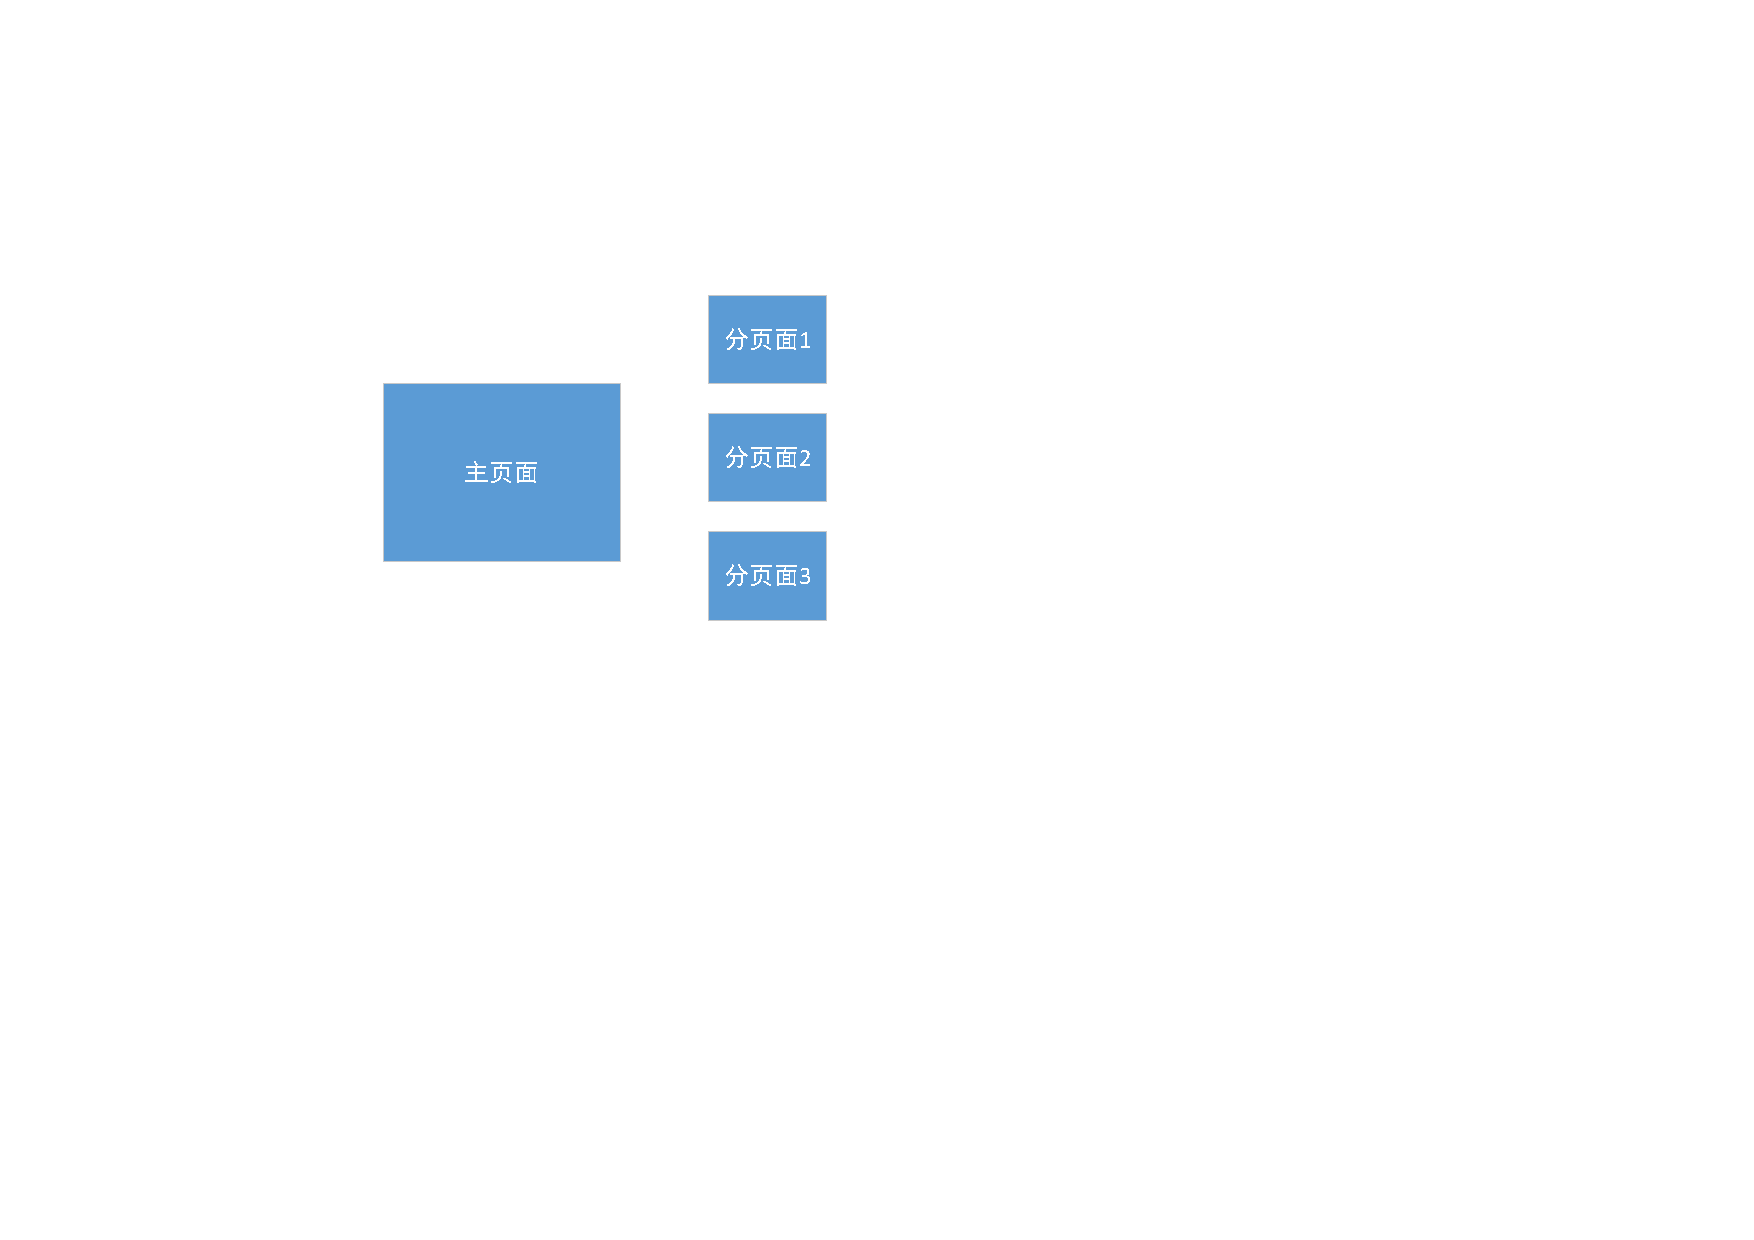
\includegraphics[scale=0.80]{images/1-1.pdf}
		\caption{网页整体框架举例}
		\label{fig2-1}
	\end{center}
\end{figure}

\subsection{实验小结}

重点说明在实验中取得的实际经验,例如调试中碰到的典型错误等,不要写套话。画图说明网页的整体框架,进行简要的文字描述等。画图说明网页的整体框架,进行简要的文字描述等。画图说明网页的整体框架,进行简要的文字描述等。画图说明网页的整体框架,进行简要的文字描述等。画图说明网页的整体框架,进行简要的文字描述等。画图说明网页的整体框架,进行简要的文字描述等。画图说明网页的整体框架,进行简要的文字描述等。

\begin{figure}[htb]
	\begin{center}
		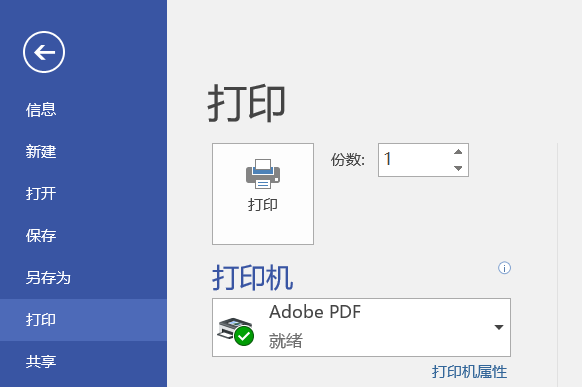
\includegraphics[scale=0.60]{images/1-2.png}
		\caption{在visio里通过文件-打印,把visio图打印成pdf文件}
		\label{fig1-2}
	\end{center}
\end{figure}

画图说明网页的整体框架,进行简要的文字描述等。画图说明网页的整体框架,进行简要的文字描述等。画图说明网页的整体框架,进行简要的文字描述等。画图说明网页的整体框架,进行简要的文字描述等。画图说明网页的整体框架,进行简要的文字描述等。画图说明网页的整体框架,进行简要的文字描述等。画图说明网页的整体框架,进行简要的文字描述等。

\begin{figure}[htb]
	\begin{center}
		
\includegraphics[scale=0.50]{images/1-3.png}
		\caption{用pdf阅览器的工具,对打印得到pdf图做适当的裁剪}
		\label{fig1-3}
	\end{center}
\end{figure}

其实吧,用Latex写公式也不是很难,请参照公式\ref{equ_loss}。画表格就更简单了,请看表\ref{table2}。

\begin{eqnarray}\label{equ_loss}
	\mathcal{L}_{id}=\sum_{j=1}^{c}1\{l_k=j\}\log\frac{\exp(f_j(\textbf{W},x_k))}{\sum\nolimits_{l=1}^{c}\exp(f_l(\textbf{W},x_k))}
\end{eqnarray}

画图说明网页的整体框架,进行简要的文字描述等。画图说明网页的整体框架,进行简要的文字描述等。画图说明网页的整体框架,进行简要的文字描述等。画图说明网页的整体框架,进行简要的文字描述等。画图说明网页的整体框架,进行简要的文字描述等。画图说明网页的整体框架,进行简要的文字描述等。画图说明网页的整体框架,进行简要的文字描述等。

\begin{table}
	\begin{center}
		\setlength{\tabcolsep}{2.0mm}
		\caption{Mean and standard deviation of estimation error (Euler angles) on Pandora. The best performance is in \textbf{bold}.}
		\label{table2}
		\begin{tabular}{c|ccccc}
			\hline
			Method                    & Data             & Pitch         & Roll          & Yaw             & Accuracy       \\
			\hline
			\hline			
			\multirow{5}{*}{POSEidon} & Depth            & 6.5 $\pm$ 6.6 & 5.4 $\pm$ 5.1 & 10.4 $\pm$ 11.8 & 0.646          \\
			                          & FfD              & 6.8 $\pm$ 7.0 & 5.7 $\pm$ 5.7 & 10.5 $\pm$ 14.6 & 0.647          \\
			                          & Gray-level       & 7.1 $\pm$ 6.6 & 5.6 $\pm$ 5.8 & 9.0  $\pm$ 10.9 & 0.639          \\
			                          & Depth + FfD      & 5.6 $\pm$ 5.0 & 4.9 $\pm$ 5.0 & 9.8  $\pm$ 13.4 & 0.698          \\
			                          & Depth + FfD + MI & 5.7 $\pm$ 5.6 & 4.9 $\pm$ 5.1 & 9.0  $\pm$ 11.9 & 0.715          \\
			\hline
			DRF                       & Depth            & 6.2 $\pm$ 9.5 & 4.6 $\pm$ 6.7 & 9.3  $\pm$ 14.6 & --             \\
			\hline
			\multirow{3}{*}{Ours}     & Depth            & 5.9 $\pm$ 6.2 & 4.5 $\pm$ 4.9 & 8.8  $\pm$ 10.9 & 0.666          \\
			                          & RGB              & 5.5 $\pm$ 5.3 & 4.4 $\pm$ 5.5 & 8.6  $\pm$ 9.3  & 0.698          \\
			                          & RGB + Depth      & 5.0 $\pm$ 4.8 & 4.3 $\pm$ 4.9 & 8.1  $\pm$ 8.3  & \textbf{0.737} \\
			\hline
		\end{tabular}
	\end{center}
\end{table}

\newpage

\section{基于链式存储结构的线性表实现}

描述主页的结构,给出主页截图,描述主要设计思路等,请见图\ref{fig2-1}。描述主页的结构,给出主页截图,描述主要设计思路等。描述主页的结构,给出主页截图,描述主要设计思路等。描述主页的结构,给出主页截图,描述主要设计思路等。描述主页的结构,给出主页截图,描述主要设计思路等。描述主页的结构,给出主页截图,描述主要设计思路等。描述主页的结构,给出主页截图,描述主要设计思路等。

\begin{figure}[htb]
	\begin{center}
		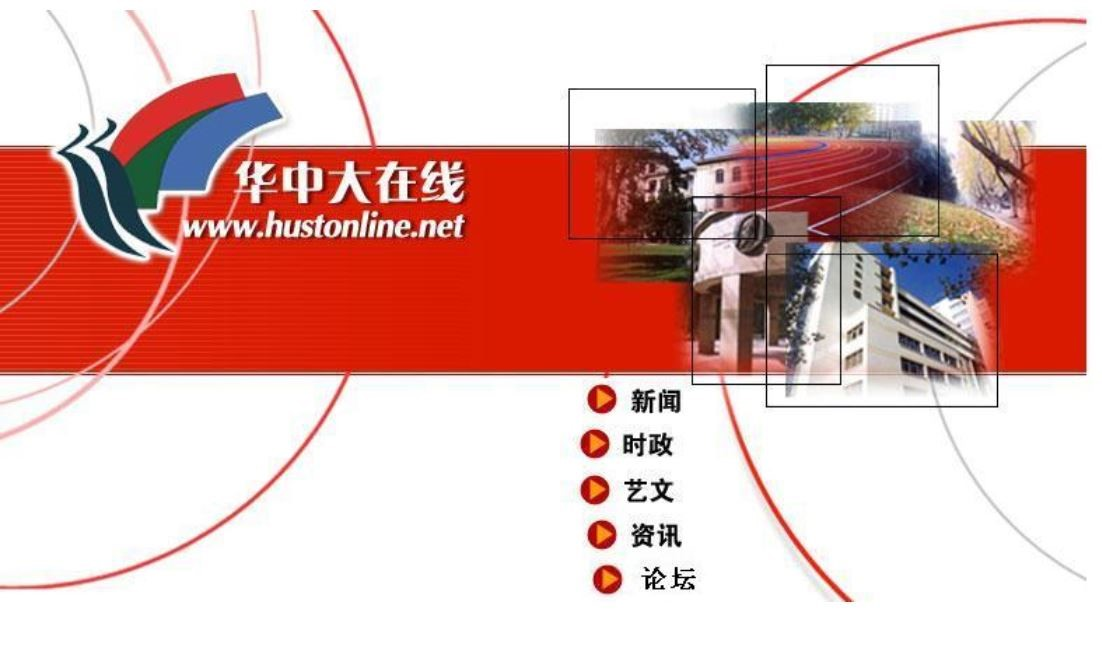
\includegraphics[scale=0.40]{images/2-1.jpg}
		\caption{主页举例}
		\label{fig2-1}
	\end{center}
\end{figure}

\subsection{问题描述}

说明此实验要解决的基本问题。大力出奇迹!!!参考文献无法显示怎么办?陈老师正在想办法解决\cite{STR2021Neurocom, AVS2021Neurocom}!我是参考文献。我是第二小节\cite{Mehrabian1974An}。我是第二小节\cite{Rezaei2014CVPR}。我是第二小节\cite{Ramnath2008IJCV}。

\subsection{系统设计}

包括整体系统结构设计和数据结构设计等。先在文件夹里的bib文件里添加新的参考文献,给每篇参考文献取一个索引的名字,然后再引用比如\cite{STR2021Neurocom}\cite{AVS2021Neurocom, Rezaei2014CVPR}。请注意书籍、期刊论文、专利等bib条目的格式是不一样的。画图说明网页的整体框架,进行简要的文字描述等。画图说明网页的整体框架,进行简要的文字描述等。画图说明网页的整体框架,进行简要的文字描述等。画图说明网页的整体框架,进行简要的文字描述等。画图说明网页的整体框架,进行简要的文字描述等。画图说明网页的整体框架,进行简要的文字描述等。画图说明网页的整体框架,进行简要的文字描述等。

\subsection{系统实现}

主要说明各个主要函数的实现思想,复杂函数可辅助流程图进行说明,函数和系统实现的源代码放在附录中。画图说明网页的整体框架,进行简要的文字描述等。画图说明网页的整体框架,进行简要的文字描述等。画图说明网页的整体框架,进行简要的文字描述等。画图说明网页的整体框架,进行简要的文字描述等。画图说明网页的整体框架,进行简要的文字描述等。画图说明网页的整体框架,进行简要的文字描述等。画图说明网页的整体框架,进行简要的文字描述等。

\subsection{系统测试}

主要说明针对各个函数正常和异常的测试用例及测试结果画图说明网页的整体框架,进行简要的文字描述等。画图说明网页的整体框架,进行简要的文字描述等。画图说明网页的整体框架,进行简要的文字描述等。画图说明网页的整体框架,进行简要的文字描述等。画图说明网页的整体框架,进行简要的文字描述等。画图说明网页的整体框架,进行简要的文字描述等。画图说明网页的整体框架,进行简要的文字描述等。

\begin{figure}[htb] % here top bottom
	\begin{center}
		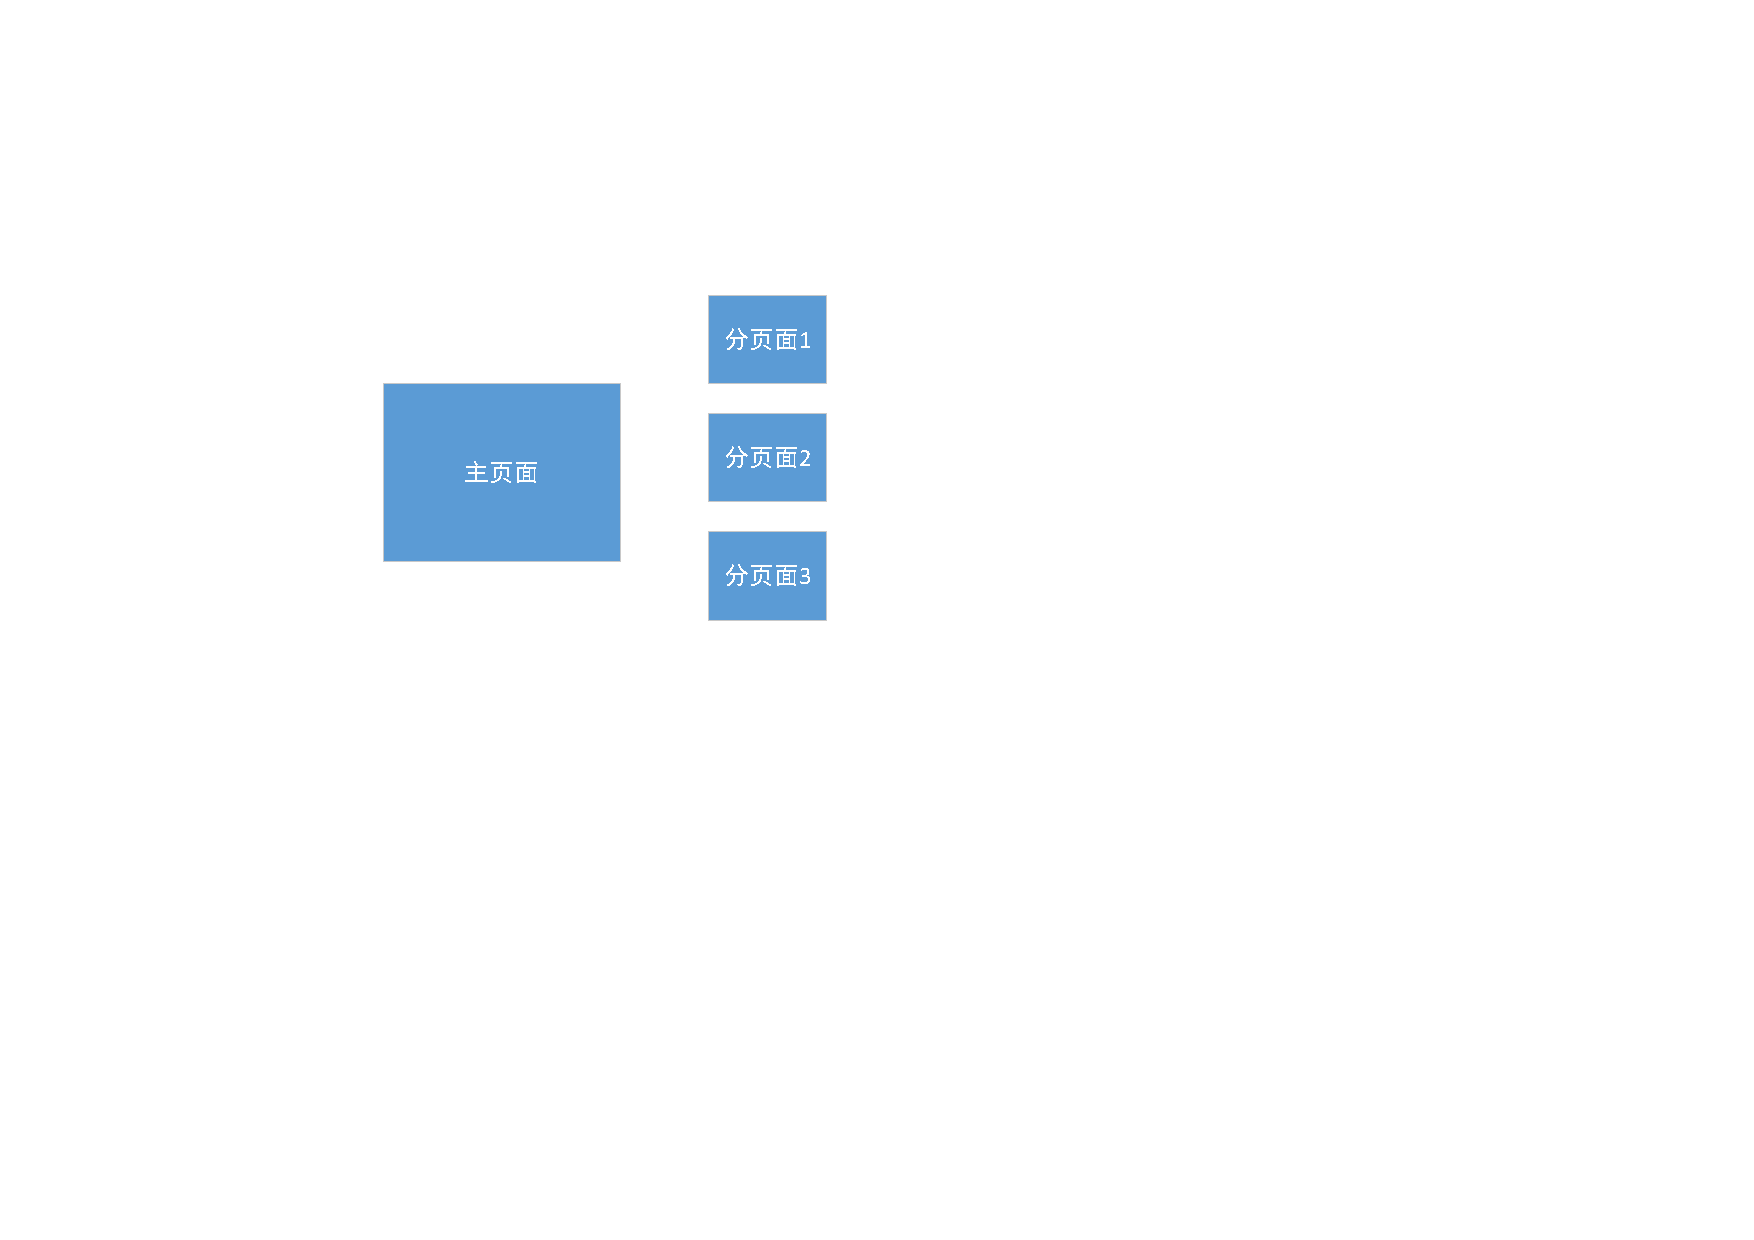
\includegraphics[scale=0.80]{images/1-1.pdf}
		\caption{网页整体框架举例}
		\label{fig4-1}
	\end{center}
\end{figure}

\subsection{实验小结}

\newpage

\section{基于二叉链表的二叉树实现}

给出分页面截图,描述主要设计思路等。给出分页面截图,描述主要设计思路等。给出分页面截图,描述主要设计思路等。给出分页面截图,描述主要设计思路等。

\subsection{问题描述}

说明此实验要解决的基本问题。大力出奇迹!!!参考文献无法显示怎么办?陈老师正在想办法解决\cite{STR2021Neurocom, AVS2021Neurocom}!我是参考文献。我是第二小节\cite{Mehrabian1974An}。我是第二小节\cite{Rezaei2014CVPR}。我是第二小节\cite{Ramnath2008IJCV}。

\subsection{系统设计}

包括整体系统结构设计和数据结构设计等。先在文件夹里的bib文件里添加新的参考文献,给每篇参考文献取一个索引的名字,然后再引用比如\cite{STR2021Neurocom}\cite{AVS2021Neurocom, Rezaei2014CVPR}。请注意书籍、期刊论文、专利等bib条目的格式是不一样的。画图说明网页的整体框架,进行简要的文字描述等。画图说明网页的整体框架,进行简要的文字描述等。画图说明网页的整体框架,进行简要的文字描述等。画图说明网页的整体框架,进行简要的文字描述等。画图说明网页的整体框架,进行简要的文字描述等。画图说明网页的整体框架,进行简要的文字描述等。画图说明网页的整体框架,进行简要的文字描述等。

\subsection{系统实现}

主要说明各个主要函数的实现思想,复杂函数可辅助流程图进行说明,函数和系统实现的源代码放在附录中。画图说明网页的整体框架,进行简要的文字描述等。画图说明网页的整体框架,进行简要的文字描述等。画图说明网页的整体框架,进行简要的文字描述等。画图说明网页的整体框架,进行简要的文字描述等。画图说明网页的整体框架,进行简要的文字描述等。画图说明网页的整体框架,进行简要的文字描述等。画图说明网页的整体框架,进行简要的文字描述等。

\subsection{系统测试}

主要说明针对各个函数正常和异常的测试用例及测试结果画图说明网页的整体框架,进行简要的文字描述等。画图说明网页的整体框架,进行简要的文字描述等。画图说明网页的整体框架,进行简要的文字描述等。画图说明网页的整体框架,进行简要的文字描述等。画图说明网页的整体框架,进行简要的文字描述等。画图说明网页的整体框架,进行简要的文字描述等。画图说明网页的整体框架,进行简要的文字描述等。

\begin{figure}[htb] % here top bottom
	\begin{center}
		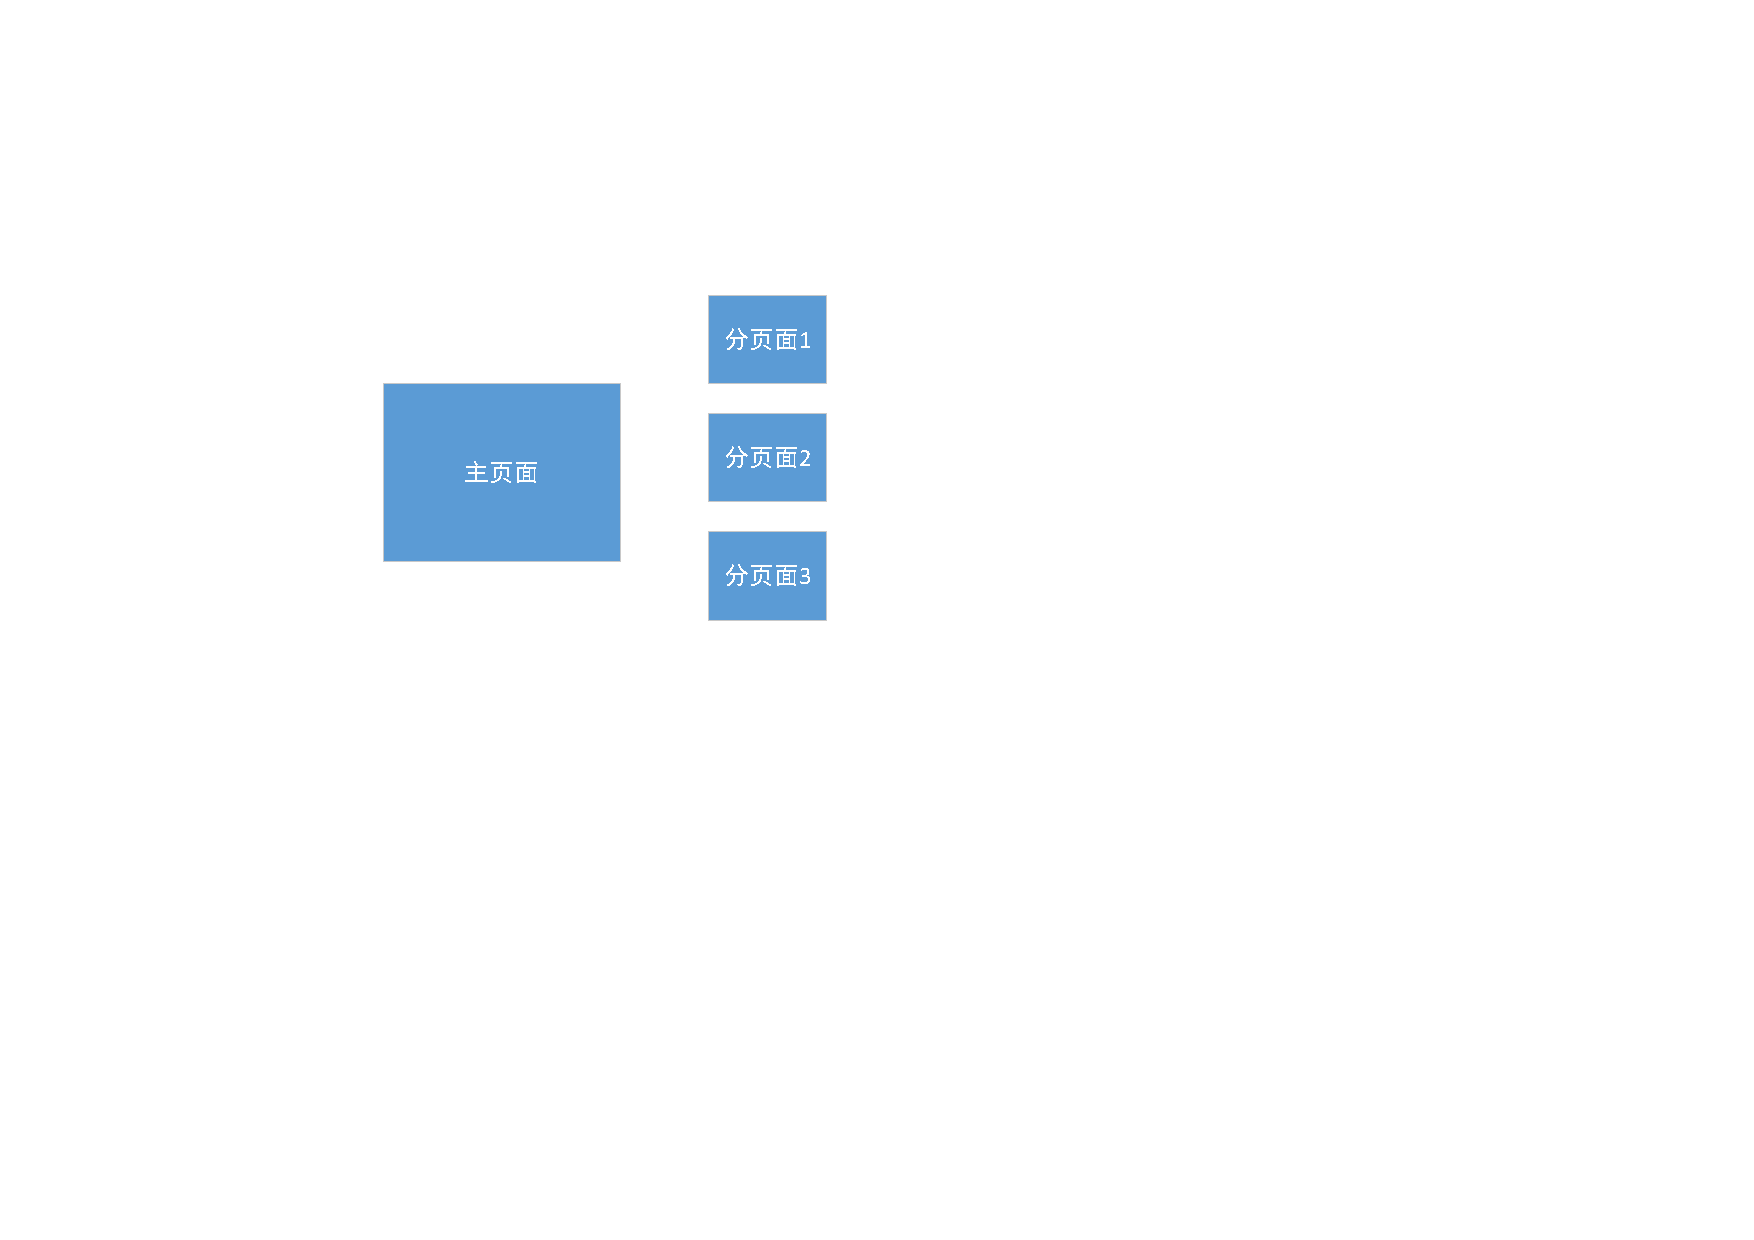
\includegraphics[scale=0.80]{images/1-1.pdf}
		\caption{网页整体框架举例}
		\label{fig3-1}
	\end{center}
\end{figure}

\subsection{实验小结}

如果实验报告中要用到算法伪代码,请参考算法\ref{alg:1},也可以参考算法\ref{alg:2}。如果实验报告中要用到算法伪代码,请参考算法\ref{alg:1},也可以参考算法\ref{alg:2}。如果实验报告中要用到算法伪代码,请参考算法\ref{alg:1},也可以参考算法\ref{alg:2}。如果实验报告中要用到算法伪代码,请参考算法\ref{alg:1},也可以参考算法\ref{alg:2}。

\begin{shaded*}\begin{alg}{一个复杂算法}
		\label{alg:1}
		\begin{algorithmic}
			\Input Two numbers $a$ and $b$
			\Output The sum of $a$ and $b$
			\Procedure{A-Plus-B}{$a, b$}
			\If $a = 0$
			\State \Return $b$
			\EndIf
			\State $res \gets 0$
			\While{$b \neq 0$}
			\State Increase $res$ by $1$
			\State $b \gets b - 1$
			\EndWhile
			\State \Return $res$
			\EndProcedure
		\end{algorithmic}
	\end{alg}\end{shaded*}

如果实验报告中要用到算法伪代码,请参考算法\ref{alg:1},也可以参考算法\ref{alg:2}。如果实验报告中要用到算法伪代码,请参考算法\ref{alg:1},也可以参考算法\ref{alg:2}。如果实验报告中要用到算法伪代码,请参考算法\ref{alg:1},也可以参考算法\ref{alg:2}。如果实验报告中要用到算法伪代码,请参考算法\ref{alg:1},也可以参考算法\ref{alg:2}。

\begin{algorithm}[h]
	\caption{一个更复杂算法}
	\begin{algorithmic}[1]
		\State Initialization: $I_{xy}$, $z_{f}=Zeros(128, 128)$; 
		\For{$0\leq n \textless N$}
		\State $i=\lfloor x_n \rfloor+64$, $j=\lfloor y_n \rfloor + 64$
		\If{$z_n<0$ and $|z_n|>|z_{f}(i,j)|$};
		\State $z_{f}(i,j)=z_n$;
		\EndIf
		\State $I_{xy}(i,j)=z_{f}(i,j)$;
		\EndFor 
	\end{algorithmic}\label{alg:2}
\end{algorithm}

\newpage

\section{基于邻接表的图实现}

\subsection{问题描述}

说明此实验要解决的基本问题。大力出奇迹!!!参考文献无法显示怎么办?陈老师正在想办法解决\cite{STR2021Neurocom, AVS2021Neurocom}!我是参考文献。我是第二小节\cite{Mehrabian1974An}。我是第二小节\cite{Rezaei2014CVPR}。我是第二小节\cite{Ramnath2008IJCV}。

\subsection{系统设计}

包括整体系统结构设计和数据结构设计等。先在文件夹里的bib文件里添加新的参考文献,给每篇参考文献取一个索引的名字,然后再引用比如\cite{STR2021Neurocom}\cite{AVS2021Neurocom, Rezaei2014CVPR}。请注意书籍、期刊论文、专利等bib条目的格式是不一样的。画图说明网页的整体框架,进行简要的文字描述等。画图说明网页的整体框架,进行简要的文字描述等。画图说明网页的整体框架,进行简要的文字描述等。画图说明网页的整体框架,进行简要的文字描述等。画图说明网页的整体框架,进行简要的文字描述等。画图说明网页的整体框架,进行简要的文字描述等。画图说明网页的整体框架,进行简要的文字描述等。

\subsection{系统实现}

主要说明各个主要函数的实现思想,复杂函数可辅助流程图进行说明,函数和系统实现的源代码放在附录中。画图说明网页的整体框架,进行简要的文字描述等。画图说明网页的整体框架,进行简要的文字描述等。画图说明网页的整体框架,进行简要的文字描述等。画图说明网页的整体框架,进行简要的文字描述等。画图说明网页的整体框架,进行简要的文字描述等。画图说明网页的整体框架,进行简要的文字描述等。画图说明网页的整体框架,进行简要的文字描述等。

\subsection{系统测试}

主要说明针对各个函数正常和异常的测试用例及测试结果画图说明网页的整体框架,进行简要的文字描述等。画图说明网页的整体框架,进行简要的文字描述等。画图说明网页的整体框架,进行简要的文字描述等。画图说明网页的整体框架,进行简要的文字描述等。画图说明网页的整体框架,进行简要的文字描述等。画图说明网页的整体框架,进行简要的文字描述等。画图说明网页的整体框架,进行简要的文字描述等。

\begin{figure}[htb] % here top bottom
	\begin{center}
		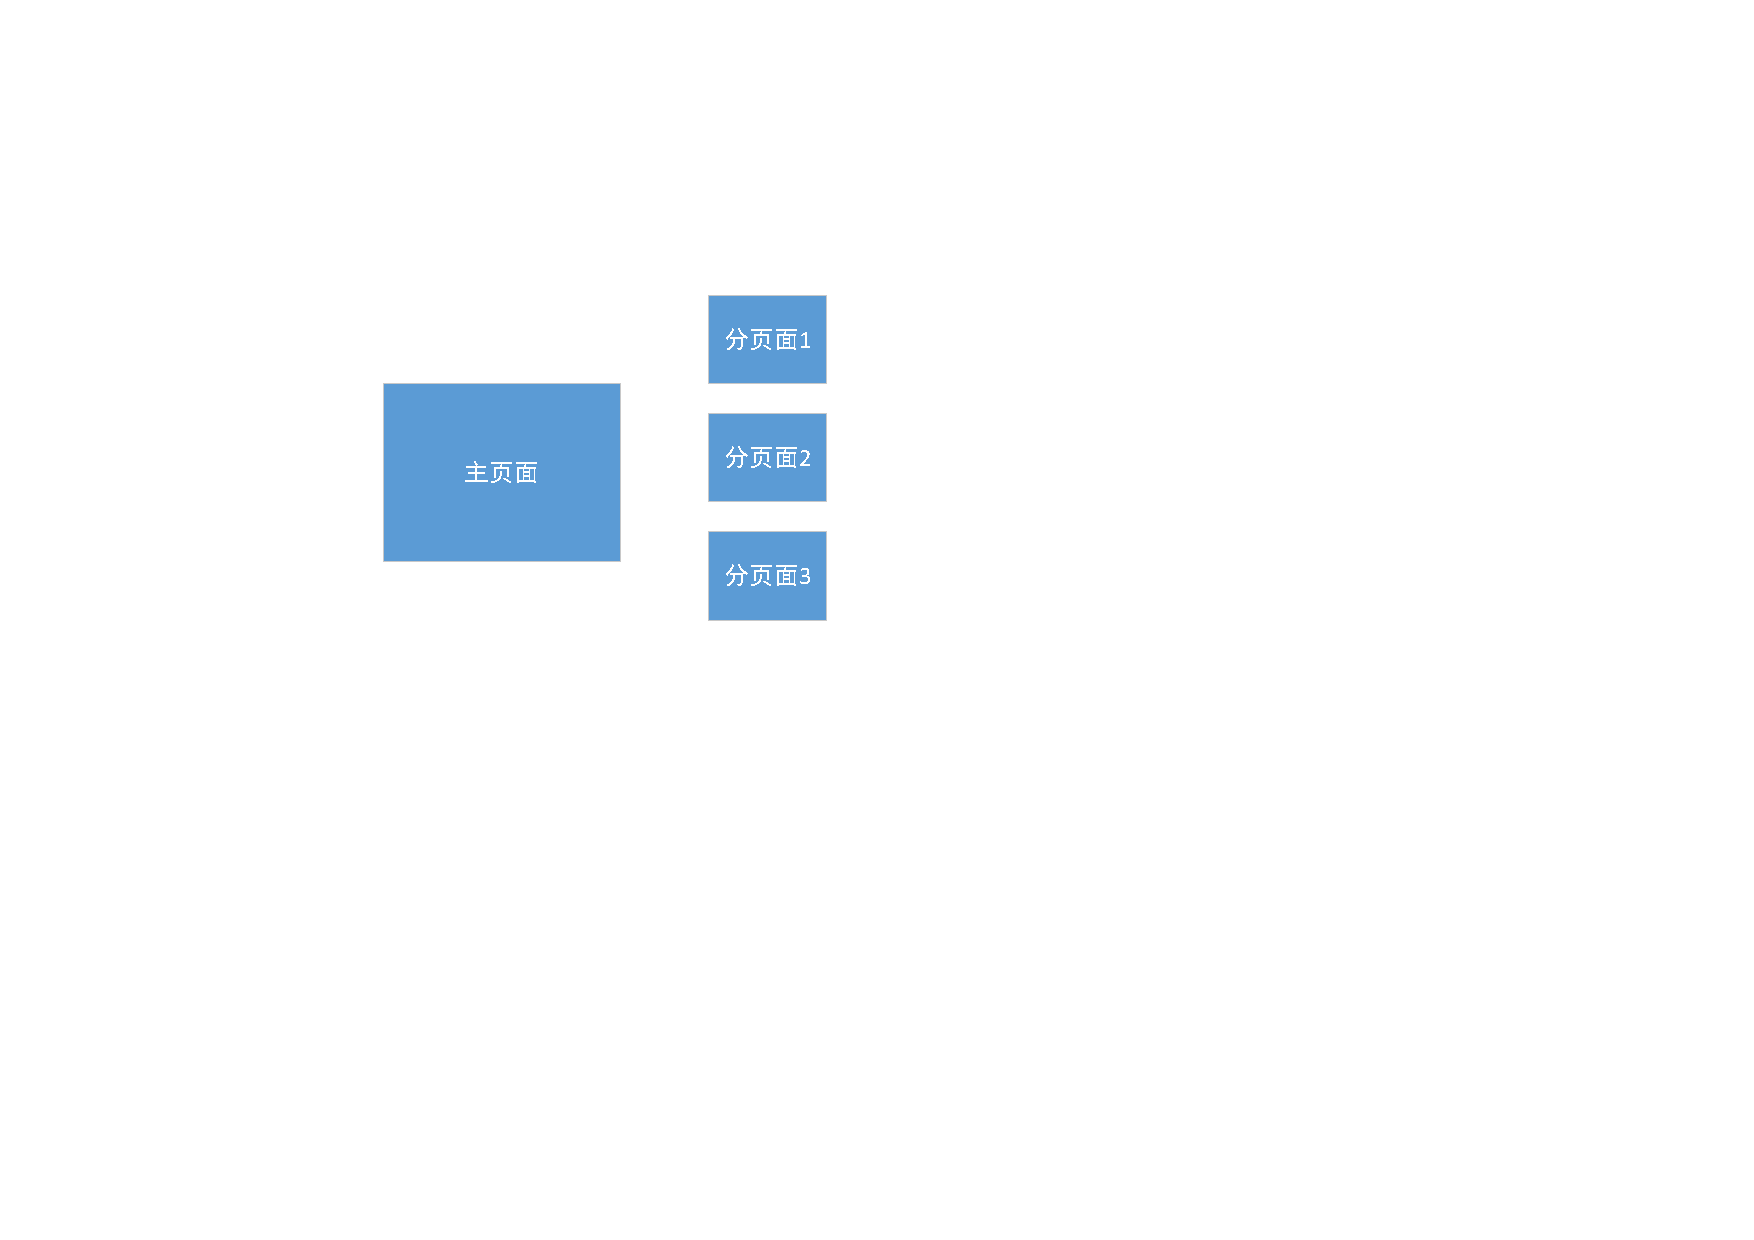
\includegraphics[scale=0.80]{images/1-1.pdf}
		\caption{网页整体框架举例}
		\label{fig5-1}
	\end{center}
\end{figure}

\subsection{实验小结}

\newpage

\section{课程的收获和建议}

描述通过学习该专题,有何收获,有何建议,如某专题可适当减少讲授时间、某专题可适当增加讲授内容和时间等。描述通过学习该专题,有何收获,有何建议,如某专题可适当减少讲授时间、某专题可适当增加讲授内容和时间等。描述通过学习该专题,有何收获,有何建议,如某专题可适当减少讲授时间、某专题可适当增加讲授内容和时间等。描述通过学习该专题,有何收获,有何建议,如某专题可适当减少讲授时间、某专题可适当增加讲授内容和时间等。

\subsection{基于顺序存储结构的线性表实现}

描述通过学习计算机基础知识专题,有何收获,有何建议,如某专题可适当减少讲授时间、某专题可适当增加讲授内容和时间等。描述网页的设计和实现过程中遇到的问题及如何解决。描述网页的设计和实现过程中遇到的问题及如何解决。描述网页的设计和实现过程中遇到的问题及如何解决。描述网页的设计和实现过程中遇到的问题及如何解决。描述网页的设计和实现过程中遇到的问题及如何解决。描述网页的设计和实现过程中遇到的问题及如何解决。描述网页的设计和实现过程中遇到的问题及如何解决。描述网页的设计和实现过程中遇到的问题及如何解决。

\subsection{基于链式存储结构的线性表实现}

描述通过学习文档撰写工具LaTeX专题,有何收获,有何建议,如某专题可适当减少讲授时间、某专题可适当增加讲授内容和时间等。描述通过学习文档撰写工具LaTeX专题,有何收获,有何建议,如某专题可适当减少讲授时间、某专题可适当增加讲授内容和时间等。

\subsection{基于二叉链表的二叉树实现}

描述通过学习编程工具Python专题,有何收获,有何建议,如某专题可适当减少讲授时间、某专题可适当增加讲授内容和时间等。描述通过学习编程工具Python专题,有何收获,有何建议,如某专题可适当减少讲授时间、某专题可适当增加讲授内容和时间等。

\subsection{基于二叉链表的二叉树实现}

描述通过学习计算机基础知识专题,有何收获,有何建议,如某专题可适当减少讲授时间、某专题可适当增加讲授内容和时间等。描述通过学习计算机基础知识专题,有何收获,有何建议,如某专题可适当减少讲授时间、某专题可适当增加讲授内容和时间等。


\nocite{*} %% 作用是不对文献进行引用,但可以生成文献列表

\bibliographystyle{sample}
\bibliography{sample}
\setcounter{secnumdepth}{0}
\appendix

\section{附录A 基于顺序存储结构线性表实现的源程序}

\noindent
/* Linear Table On Sequence Structure */\\
\#include <stdio.h>\\
\#include <malloc.h>\\
\#include <stdlib.h>\\

\noindent
/*---------page 10 on textbook ---------*/\\
\#define TRUE 1\\
\#define FALSE 0\\
\#define OK 1\\
\#define ERROR 0\\
\#define INFEASTABLE -1\\
\#define OVERFLOW -2\\
\newpage
\section{附录B 基于链式存储结构线性表实现的源程序}
\newpage
\section{附录C 基于二叉链表二叉树实现的源程序}
\newpage
\section{附录D 基于邻接表图实现的源程序}

\end{document}